\section{Algorithm \& Implementation}
\label{sec:algorithm_implementation}
% TODO: Description or something

\subsection{Equation Solving}
\label{subsec:equation_solving}
Before we delve into the actual algorithms we need to cover a problem that lies at the core of the procedures which we call the \emph{line segment intersection problem}. 
\begin{definition}[Line Segment Intersection Problem]
  Let \(e = \overline{e_1e_2}\) be a \(d\)-dimensional line segment, \(u \in \R^d\) be a point, \(\varepsilon > 0\) and \(\delta\) a distance function. In the \emph{line segment intersection problem} we are interested in determining the set \(\set{t \in [0, 1] \mid \delta(e_1 + t(e_2 - e_1), u) \leq \varepsilon}\).

  As the name suggests, this corresponds to the intersection of \(\set{x \in \R^d \mid \delta(x, u) \leq \varepsilon}\), the set of points with distance at most \(\varepsilon\) from \(u\), and the line segment. 
\end{definition}

\begin{observation}
  For \(\ell \in [1, \infty]\) the solution set to the line segment intersection problem using the distance \(\delta_\ell\) is convex. Thus we can write it as a single interval \(I \subseteq [0, 1]\). This interval is either empty or it is closed allowing us to identify it via the left and right boundary of the interval. 
\end{observation}
\begin{proof}
  Follows directly from property 3 of \cref{lem:distance_properties} and the fact that intervals and the points on line segments are convex sets. 
\end{proof}

This simplifies the finding of these sets to only determining the boundaries, or determine that the interval is empty. For this, we solve equations involving distance functions \(\delta\). More specifically, we want to solve the following equation of the bounding points
\begin{equation}
  \delta(u + t \cdot (v - u), w) = \varepsilon \label{eq:eq_solve_main}
\end{equation}
for arbitrary, fixed vectors \(u, v, w \in \R^d\) and fixed \(\varepsilon \in \R_{>0}\) for the variable \(t \in \R\) or determine that there is no such solution. This corresponds to the points the lie on the line segment \(e = \overline{uv}\) that have distance \(\varepsilon\) from \(w\) as each point on \(e\) is of the form \(u + t(v-u)\). 

We label the smallest solution of \cref{eq:eq_solve_main} \(\hat{t}_0\) and the largest solution \(\hat{t}_1\). Note that these may not be the solutions the line segment intersection problem as the solutions may be outside of the interval \([0, 1]\). Those two solutions may be the same, i.e, the interval collapses to a single point, or may not exist at all, meaning the interval is empty.

We need to modify the solutions \(\hat{t}_0\) and \(\hat{t}_1\) to the actual solutions \(\hat{t}_0'\) and \(\hat{t}_1'\) which can be defined as 
\begin{equation}
  \hat{t}_0' \coloneq \begin{cases}
    0 & \textrm{ if } \hat{t}_0 < 0 \textrm{ and } \hat{t}_1 \geq 0\\
    \hat{t}_0 & \textrm{ if } \hat{t}_0 \in [0, 1]\\
    \infty &\textrm{ otherwise }
  \end{cases}\\
  \hat{t}_1' \coloneq \begin{cases}
    1 & \textrm{ if } \hat{t}_1 > 1 \textrm{ and } \hat{t}_0 \leq 1\\
    \hat{t}_1 & \textrm{ if } \hat{t}_1 \in [0, 1]\\

    \infty &\textrm{ otherwise }
  \end{cases},
\end{equation}
where the \emph{otherwise} case also includes the case of there being no solution to \cref{eq:eq_solve_main}. This corresponds to the smallest and largest point in the modified interval \([\hat t_0, \hat t_1] \cap [0, 1]\) which is the actual solution to the line segment intersection problem. \cref{fig:solution_kinds} shows how this affects the solutions.
For a line segment \(\overline{uv}\) and a point \(w\) we denote \(\hat t_0'(\overline{uv}, w)\) and \(\hat t_1'(\overline{uv}, w)\) to be the respective modified solutions for the given line segment and point. We do not include \(\varepsilon\) in that notation as it is fixed throughout all algorithms and thus requires no disambiguation.

\begin{figure}
    \centering
    % First row of subfigures
    \begin{subfigure}[b]{0.3\textwidth}
        \centering
        \begin{tikzpicture}
            % Define points
            \coordinate (u)  at (2,0.5);
            \coordinate (u0) at (0,0);
            \coordinate (v) at (4,1);
            \coordinate (w) at (2,0);

            % Draw the line segment from u to v
            \draw[thick] (u) -- (v);

            \draw[thick] (w) circle (1);

            % Find intersection points between the line and the circle
            \path[name path=line] (u0) -- (v);
            \path[name path=circle] (w) circle (1);
            \path[name intersections={of=line and circle, by={t1,t0}}];

            % Label intersection points
            \node[circle,fill,color=red,inner sep=1pt,label={[text=red, below]:\(u=\hat t_0'\)}] at (u) [] {}; 
            \node[circle,fill,color=blue,inner sep=1pt,label={[text=blue]-90:\(v\)}] at (v) [] {}; 
            \node[circle,fill,color=blue,inner sep=1pt,label={[text=blue]-90:\(w\)}] at (w) [] {}; 

            \node[circle,fill,color=red,inner sep=1pt,label={[text=red, above left]:\(\hat t_0\)}] at (t0) [] {}; 
            \node[circle,fill,color=red,inner sep=1pt,label={[text=red, above]:\(\hat t_1=\hat t_1'\)}] at (t1) [] {}; 

            % Draw dotted extensions of the line segment
            \draw[dotted] (u0) -- (u);
            %\draw[dotted] (v) -- ($(v)!-1.5!(u)$);
        \end{tikzpicture}
      \caption{\(\hat t_0 < 0 < \hat t_1 < 1\) \\ \(\hat t_0' = 0, \hat t_1' = \hat t_1\)}
    \end{subfigure}
    \hfill
    \begin{subfigure}[b]{0.3\textwidth}
        \centering
        \begin{tikzpicture}
            % Define points
            \coordinate (u) at (0,0);
            \coordinate (v) at (4,1);
            \coordinate (w) at (2,0);

            % Draw the line segment from u to v
            \draw[thick] (u) -- (v);

            \draw[thick] (w) circle (1);

            % Find intersection points between the line and the circle
            \path[name path=line] (u) -- (v);
            \path[name path=circle] (w) circle (1);
            \path[name intersections={of=line and circle, by={t1,t0}}];

            % Label intersection points
            \node[circle,fill,color=blue,inner sep=1pt,label={[text=blue]-90:\(u\)}] at (u) [] {}; 
            \node[circle,fill,color=blue,inner sep=1pt,label={[text=blue]-90:\(v\)}] at (v) [] {}; 
            \node[circle,fill,color=blue,inner sep=1pt,label={[text=blue]-90:\(w\)}] at (w) [] {}; 

            \node[circle,fill,color=red,inner sep=1pt,label={[text=red, above left]:\(\hat t_0=\hat t_0'\)}] at (t0) [] {}; 
            \node[circle,fill,color=red,inner sep=1pt,label={[text=red, above]:\(\hat t_1=\hat t_1'\)}] at (t1) [] {}; 

            % Draw dotted extensions of the line segment
            %\draw[dotted] ($(u)!-1.5!(v)$) -- (u);
            %\draw[dotted] (v) -- ($(v)!-1.5!(u)$);
        \end{tikzpicture}
        \caption{\(0 < \hat t_0 < \hat t_1 < 1\)\\ \(\hat t_0' = \hat t_0, \hat t_1' = \hat t_1\)}
    \end{subfigure}
    \hfill
    \begin{subfigure}[b]{0.3\textwidth}
        \centering
        \begin{tikzpicture}
            % Define points
            \coordinate (v)  at (2,0.5);
            \coordinate (u) at (0,0);
            \coordinate (v0) at (4,1);
            \coordinate (w) at (2,0);

            % Draw the line segment from u to v
            \draw[thick] (u) -- (v);

            \draw[thick] (w) circle (1);

            % Find intersection points between the line and the circle
            \path[name path=line] (u) -- (v0);
            \path[name path=circle] (w) circle (1);
            \path[name intersections={of=line and circle, by={t1,t0}}];

            % Label intersection points
            \node[circle,fill,color=blue,inner sep=1pt,label={[text=blue, below]:\(u\)}] at (u) [] {}; 
            \node[circle,fill,color=red,inner sep=1pt,label={[text=red, below]:\(v=\hat t_1'\)}] at (v) [] {}; 
            \node[circle,fill,color=blue,inner sep=1pt,label={[text=blue]-90:\(w\)}] at (w) [] {}; 

            \node[circle,fill,color=red,inner sep=1pt,label={[text=red, above left]:\(\hat t_0=\hat t_0'\)}] at (t0) [] {}; 
            \node[circle,fill,color=red,inner sep=1pt,label={[text=red, above]:\(\hat t_1\)}] at (t1) [] {}; 

            % Draw dotted extensions of the line segment
            \draw[dotted] (v) -- (v0);
            %\draw[dotted] (v) -- ($(v)!-1.5!(u)$);
        \end{tikzpicture}
      \caption{\(0 < \hat t_0 < 1 < \hat t_1 \) \\ \(\hat t_0' = \hat t_0, \hat t_1' = 1\)}
    \end{subfigure}

    % Second row of subfigures
    \begin{subfigure}[b]{0.3\textwidth}
        \centering
        \begin{tikzpicture}
            % Define points
            \coordinate (u) at (0,0);
            \coordinate (v0) at (4,1);
            \coordinate (v) at (2,0.5);
            \coordinate (w) at (3,0);

            % Draw the line segment from u to v
            \draw[thick] (u) -- (v);

            \draw[thick] (w) circle (1);

            % Find intersection points between the line and the circle
            \path[name path=line] (u) -- (v0);
            \path[name path=circle] (w) circle (1);
            \path[name intersections={of=line and circle, by={t1,t0}}];

            % Label intersection points
            \node[circle,fill,color=blue,inner sep=1pt,label={[text=blue]-90:\(u\)}] at (u) [] {}; 
            \node[circle,fill,color=blue,inner sep=1pt,label={[text=blue, above]:\(v\)}] at (v) [] {}; 
            \node[circle,fill,color=blue,inner sep=1pt,label={[text=blue]-90:\(w\)}] at (w) [] {}; 

            \node[circle,fill,color=red,inner sep=1pt,label={[text=red, below right]:\(\hat t_0\)}] at (t0) [] {}; 
            \node[circle,fill,color=red,inner sep=1pt,label={[text=red, above]:\(\hat t_1\)}] at (t1) [] {}; 

            % Draw dotted extensions of the line segment
            \draw[dotted] (v) -- (v0);
            %\draw[dotted] (v) -- ($(v)!-1.5!(u)$);
        \end{tikzpicture}
        \caption{\(\hat t_0 < \hat t_1 < 0\)\\ \(\hat t_0' = \hat t_1' = \infty\)}
    \end{subfigure}
    \hfill
    \begin{subfigure}[b]{0.3\textwidth}
        \centering
        \begin{tikzpicture}
            % Define points
            \coordinate (u0) at (-1.5,-0.5);
            \coordinate (u) at (-0.75,-0.125);
            \coordinate (v) at (0.5,0.5);
            \coordinate (v0) at (1.5,1);
            \coordinate (w) at (0,0);

            % Draw the line segment from u to v
            \draw[thick] (u) -- (v);

            \draw[thick] (w) circle (1);

            % Find intersection points between the line and the circle
            \path[name path=line] (u0) -- (v0);
            \path[name path=circle] (w) circle (1);
            \path[name intersections={of=line and circle, by={t1,t0}}];

            % Label intersection points
            \node[circle,fill,color=red,inner sep=1pt,label={[text=red, below right]:\(u=\hat t_0'\)}] at (u) [] {}; 
            \node[circle,fill,color=red,inner sep=1pt,label={[text=red, left]:\(v=\hat t_1'\)}] at (v) [] {}; 
            \node[circle,fill,color=blue,inner sep=1pt,label={[text=blue,right]:\(w\)}] at (w) [] {}; 

            \node[circle,fill,color=red,inner sep=1pt,label={[text=red, left]:\(\hat t_0\)}] at (t0) [] {}; 
            \node[circle,fill,color=red,inner sep=1pt,label={[text=red, right]:\(\hat t_1\)}] at (t1) [] {}; 

            % Draw dotted extensions of the line segment
            \draw[dotted] (u0) -- (v0);
        \end{tikzpicture}
        \caption{\(\hat t_0 < 0 < 1 < \hat t_1\)\\ \(\hat t_0' = 0, \hat t_1' = 1\)}
    \end{subfigure}
    \hfill
    \begin{subfigure}[b]{0.3\textwidth}
        \centering
        \begin{tikzpicture}
            % Define points
            \coordinate (u0) at (-2,-1);
            \coordinate (u) at (1,0.5);
            \coordinate (v) at (2,1);
            \coordinate (w) at (-0.5,0);

            % Draw the line segment from u to v
            \draw[thick] (u) -- (v);

            \draw[thick] (w) circle (1);

            \path[name path=line] (u0) -- (v);
            \path[name path=circle] (w) circle (1);
            \path[name intersections={of=line and circle, by={t1,t0}}];

            \node[circle,fill,color=blue,inner sep=1pt,label={[text=blue]-90:\(u\)}] at (u) [] {}; 
            \node[circle,fill,color=blue,inner sep=1pt,label={[text=blue, above]:\(v\)}] at (v) [] {}; 
            \node[circle,fill,color=blue,inner sep=1pt,label={[text=blue]-90:\(w\)}] at (w) [] {}; 

            \node[circle,fill,color=red,inner sep=1pt,label={[text=red, below left]:\(\hat t_0\)}] at (t0) [] {}; 
            \node[circle,fill,color=red,inner sep=1pt,label={[text=red, left]:\(\hat t_1\)}] at (t1) [] {}; 

            \draw[dotted] (u) -- (u0);
        \end{tikzpicture}
        \caption{\(1 < \hat t_0 < \hat t_1\)\\ \(\hat t_0' =  \hat t_1' = \infty\)}
    \end{subfigure}

    % Third row of subfigures (centered)
    \begin{subfigure}[b]{0.3\textwidth}
        \centering
        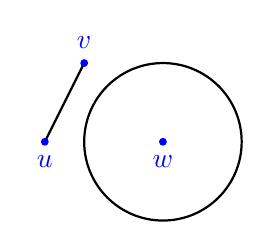
\begin{tikzpicture}
            % Define points
            \coordinate (u) at (1.5,0);
            \coordinate (v) at (2,1);
            \coordinate (w) at (3,0);

            % Draw the line segment from u to v
            \draw[thick] (u) -- (v);

            \draw[thick] (w) circle (1);

            % Label intersection points
            \node[circle,fill,color=blue,inner sep=1pt,label={[text=blue]-90:\(u\)}] at (u) [] {}; 
            \node[circle,fill,color=blue,inner sep=1pt,label={[text=blue, above]:\(v\)}] at (v) [] {}; 
            \node[circle,fill,color=blue,inner sep=1pt,label={[text=blue]-90:\(w\)}] at (w) [] {}; 
        \end{tikzpicture}
        \caption{\(\hat t_0, \hat t_1\) do not exist\\ \(\hat t_0' = \hat t_1' = \infty\)}
    \end{subfigure}
    \caption{The different kinds of solutions. Note that we associate \(0\) with \(u\), \(1\) with \(v\) and \(t\) with \((1-t)u + tv\)}
    \label{fig:solution_kinds}
\end{figure}

In general, determining these solutions requires finding roots of polynomials and thus there is no exact solution algorithm for Minkowski distances \(\delta_e\) for \(e > 4\) as such polynomials are not solvable. Here, we derive explicit solutions for the Euclidean Distance, the Manhattan Distance and the Chebyshev Distance. 

\subsubsection{Euclidean Distance}
\label{subsubsec:eq_euclidean_distance}
In the case of the Euclidean distance, \cref{eq:eq_solve_main} simplifies to the equation 
\begin{align*}
  \| (u - w) + t(v - u) \|_2 &= \varepsilon \\
  \| (u - w) + t(v - u) \|_2^2 &= \varepsilon^2 \\
  \| u - w \|_2^2 + 2\braket{u - w | v - u} t  +  \| v - u \|_2^2 t^2 &= \varepsilon^2 \\
  \underbrace{\delta(u,w)^2 - \varepsilon^2}_{\alpha_0} + \underbrace{2\braket{u - w | v - u} }_{\alpha_1}t  +  \underbrace{\delta(v, u)^2}_{\alpha_2} t^2 &= 0 \\
  \alpha_0 + \alpha_1 t  + \alpha_2 t^2 &= 0,
\end{align*}

which is a quadratic equation in \(t\) and can be solved explicitly as 

\begin{equation}
  t_{0,1} = \frac{-\alpha_1 \pm \sqrt{\alpha_1^2 - 4\alpha_0\alpha_2}}{2\alpha_2}.\label{eq:sol_explicit_euclidean}
\end{equation}

If the discriminant \(\alpha_1^2 - 4\alpha_0\alpha_2\) is smaller than \(0\) there is no solution. Otherwise we can compute the two solutions and have the smallest and largest solution. 


\subsubsection{Manhattan Distance}
\label{subsubsec:eq_manhattan_distance}
In the case of the Manhattan distance, \cref{eq:eq_solve_main} simplifies to 
\begin{equation}
  \sum_{i=0}^d |u_i - w_i + t (v_i - u_i)| = \varepsilon. \label{eq:solve_manhattan}
\end{equation}

For the Manhattan and Chebyshev distance we will use the following fact about the distance functions we have seen. 
\begin{observation}\label{obs:permute-coordinates}
  Let \(u, v \in \R^d\) and \(\sigma: \set{1, \dots, d} \to \set{1, \dots, d}\) a permutation. We define \(\sigma(u) \in \R^d\) as the vector gotten from \(u\) by permutation of the coordinates according to \(\sigma\), meaning \(\sigma(u)_i = u_{\sigma(i)}\) for \(i \in \set{1, \dots, d}\). Then \(\delta_\ell(u, v) = \delta_\ell(\sigma(u), \sigma(v))\) for any \(\ell \in [1, \infty]\).
\end{observation}

We note that \(|u_i - w_i + t (v_i - u_i )|\) can only assume the two values \(u_i - w_i + t(v_i - u_i)\) or \(w_i - u_i - t(v_i - u_i)\) depending on \(t\). For a fixed \(t\) we can evaluate all terms in the sum in \cref{eq:solve_manhattan} to get a linear equation in \(t\) which is trivial to solve, and the check if the resulting solution is valid. We define \(t_i \coloneq \frac{w_i - u_i}{v_i - u_i} \). Let \(\sigma:\set{1,\dots, d} \to \set{1,\dots, d}\) be the sorting permutation with \(t_{\sigma(1)} < t_{\sigma(2)} < \cdots < t_{\sigma(d)}\). Applying this permutation to both vectors \(u-w\) and \(v -u\) does not affect the distance according to \cref{obs:permute-coordinates}. For \(t \in [t_{\sigma(i)}, t_{\sigma(i+1)}]\) each of the terms in the sum can be simplified to a linear term without the absolute value and thus the whole sum degenerates into a linear equation which can be trivially solved. Finally we can check if the solution found for this interval does indeed lie in the interval. 

This whole process can be implemented na\"ively using a Sweepline algorithm in time \(\O(d^2)\) by constructing the values \(t_i\), sorting them and for each interval we compute the whole sum in linear time and solve the equation. As there are \(d\) many such values to consider we get quadratic runtime. We can improve this by using the fact that by iterating from smallest to largest during each testing step only a single term changes its sign, thus we can maintain the current linear equation and update it accordingly in constant time. The bulk of the computation now lies in sorting which gives us a runtime og \(\O(d \log d)\). 

There are a few edge cases, namely those being that multiple \(t_i\) coincide as well as that there are \(u_i = v_i\). The former case actually does not require special treatment as it will result in checking for a solution in an interval that contains only one value and at this value all with the same \(t_i\) will be zero. The second case degenerates the term into a constant which can be pulled out of the sum and into the right side.

\begin{algorithm}[ht]
  \DontPrintSemicolon
  \KwData{vectors \(u, v, w \in \R^d\), \(\varepsilon > 0\)}
  \KwResult{Solution to \cref{eq:solve_manhattan}}
  \BlankLine
  \(global\_slope \gets 0, global\_offset \gets 0\) \;
  \(events \gets Array(d)\)
  \For{\(i = 1, \dots, d\)}{
    \(slope \gets v_i - u_i, offset \gets u_i - w_i\)\;
    \If{\(slope < 0\)}{
      \(slope \gets -slope, offset \gets -offset\)
    } \ElseIf{\(slope = 0\)}{
      \(\varepsilon \gets \varepsilon - |offset|\)\;
      \Continue
    }
    \(zero \gets - \frac{offset}{slope}\)\;
    \If{\(zero \leq 0\)}{
      \(global\_offset \gets global\_offset + offset\)\;
      \(global\_slope \gets global\_slope + slope\)\;
      \Continue
    } 
    \(global\_offset \gets global\_offset - offset\)\;
    \(global\_slope \gets global\_slope - slope\)\;
    \If{\(zero \geq 1\)}{
      \Continue
    }
    \(events.append((zero, slope, offset))\)\;
  }
  Sort \(events\) by their \(zero\) component\;
  \(start \gets 0\)\;
  \For{\((zero, slope, offset) \in events\)}{
    Test if solution \(\frac{\varepsilon - global\_offset}{global\_slope} \in [start, zero]\) and report solution if so\;
    \(global\_offset \gets global\_offset + 2offset\)\;
    \(global\_slope \gets global\_slope + 2slope\)\;
    \(start \gets zero\)
  }
  Test if solution \(\frac{\varepsilon - global\_offset}{global\_slope} \in [start, 1]\) and report solution if so\;

  \caption{manhattan\_solver(\(u, v, w, \varepsilon\))}
  \label{algo:solve_manhattan}
\end{algorithm}


\subsubsection{Chebyshev Distance}
\label{subsubsec:eq_chebyshev_distance}
In the case of the Chebyshev distance \cref{eq:eq_solve_main} becomes 
\begin{equation}
  \max_{i = 1,\dots, d} |u_i - w_i + t(v_i - u_i)| = \varepsilon\label{eq:solve_chebyshev}
\end{equation}
for which a na\"ive solution can be found easily as the maximum will only assume as value one of the terms and each term has two possible values depending on the absolute value. Thus there are \(2d\) possible solutions which can be checked each in linear time if they indeed are the maximum resulting in a simple quadratic runtime algorithm. 

Just as in the case of the Manhattan distance, we only need to consider the solutions in the interval \([0,1]\) which eliminates possible solutions and in small dimensions this is probably the best choice. 

We can also reduce the runtime to \(d \log d\) by efficiently updating the current maximum. As each term is a line, we can find the initial maximum line at the start and update it when it crosses another line thus a modified version of the Bentley-Ottmann algorithm for line segment intersection (e.g. as explained in \cite{computational_geometry}) can be used where where the handling of intersections is modified to remove the line segment that falls below the other and only computing new intersections upwards. This guarantees that even if there are quadratically many intersecions only \(\O(d \log d)\) runtime is needed as irrelevant intersections are omitted. 
This allows a simplification in that we do not need a self-balancing binary search tree to store the line segments. A doubly linked list suffices as we remove for each intersection a line segment and the relative ordering remains the same. This list can be stored in an array where each array entry has an index to the previous and next line segment and its data, i.e., the offset and slope. A more detailed version of this idea can be seen in \cref{algo:solve_chebyshev} an example of the resulting line segment intersection problem can be seen in \cref{fig:chebyshev_algo}. For a full implementation, the case distinction in \cref{subsec:equation_solving} needs to be implemented, the handling of the marked solutions.

\begin{figure}
  \centering 
  \begin{subfigure}[ht]{0.3\textwidth}
    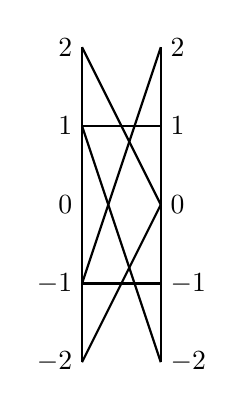
\begin{tikzpicture}
      % Draw the y-axes at x = 0 and x = 1
      \draw[thick] (0, -2) -- (0, 2) node[above] {};
      \draw[thick] (1, -2) -- (1, 2) node[above] {};

      % Add labels for the y-axis ticks
      \foreach \y in {-2, -1, 0, 1, 2} {
          \node[left] at (0, \y) {$\y$};
          \node[right] at (1, \y) {$\y$};
      }

      \draw[thick] (0,2) -- (1,0) node {};
      \draw[thick] (0,-2) -- (1,0) node {};
      \draw[thick] (0,1) -- (1,1) node {};
      \draw[thick] (0,-1) -- (1,-1) node {};
      \draw[thick] (0,-1) -- (1,2) node {};
      \draw[thick] (0,1) -- (1,-2) node {};
    \end{tikzpicture}
    \caption{All candidate lines}
  \end{subfigure}
  \begin{subfigure}[ht]{0.3\textwidth}
    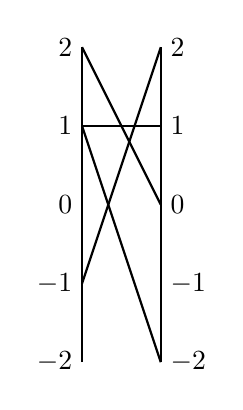
\begin{tikzpicture}
      % Draw the y-axes at x = 0 and x = 1
      \draw[thick] (0, -2) -- (0, 2) node[above] {};
      \draw[thick] (1, -2) -- (1, 2) node[above] {};

      % Add labels for the y-axis ticks
      \foreach \y in {-2, -1, 0, 1, 2} {
          \node[left] at (0, \y) {$\y$};
          \node[right] at (1, \y) {$\y$};
      }

      \draw[thick] (0,2) -- (1,0) node {};
      \draw[thick] (0,1) -- (1,1) node {};
      \draw[thick] (0,-1) -- (1,2) node {};
      \draw[thick] (0,1) -- (1,-2) node {};
    \end{tikzpicture}
    \caption{Lines that are not fully negative}
  \end{subfigure}
  \begin{subfigure}[ht]{0.3\textwidth}
    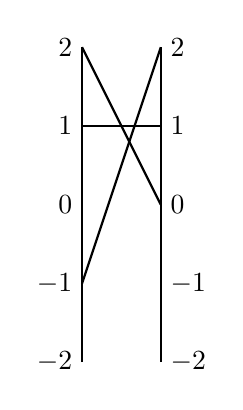
\begin{tikzpicture}
      % Draw the y-axes at x = 0 and x = 1
      \draw[thick] (0, -2) -- (0, 2) node[above] {};
      \draw[thick] (1, -2) -- (1, 2) node[above] {};

      % Add labels for the y-axis ticks
      \foreach \y in {-2, -1, 0, 1, 2} {
          \node[left] at (0, \y) {$\y$};
          \node[right] at (1, \y) {$\y$};
      }

      \draw[thick] (0,2) -- (1,0) node {};
      \draw[thick] (0,1) -- (1,1) node {};
      \draw[thick] (0,-1) -- (1,2) node {};
    \end{tikzpicture}
    \caption{Lines that are not fully below another line}
  \end{subfigure}\\
  \begin{subfigure}[ht]{0.3\textwidth}
    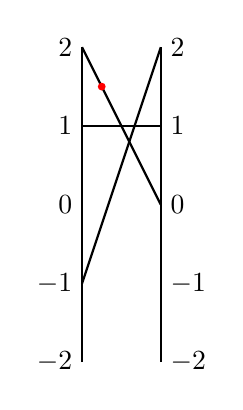
\begin{tikzpicture}
      % Draw the y-axes at x = 0 and x = 1
      \draw[thick] (0, -2) -- (0, 2) node[above] {};
      \draw[thick] (1, -2) -- (1, 2) node[above] {};

      % Add labels for the y-axis ticks
      \foreach \y in {-2, -1, 0, 1, 2} {
          \node[left] at (0, \y) {$\y$};
          \node[right] at (1, \y) {$\y$};
      }

      \draw[thick] (0,2) -- (1,0) node {};
      \draw[thick] (0,1) -- (1,1) node {};
      \draw[thick] (0,-1) -- (1,2) node {};

      \node[circle,fill,color=red,inner sep=1pt] at (0.25, 1.5) {};
    \end{tikzpicture}
    \caption{Find next intersection. Here between topmost line so check for solution.}
  \end{subfigure}
  \begin{subfigure}[ht]{0.3\textwidth}
    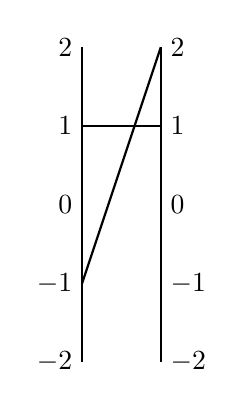
\begin{tikzpicture}
      % Draw the y-axes at x = 0 and x = 1
      \draw[thick] (0, -2) -- (0, 2) node[above] {};
      \draw[thick] (1, -2) -- (1, 2) node[above] {};

      % Add labels for the y-axis ticks
      \foreach \y in {-2, -1, 0, 1, 2} {
          \node[left] at (0, \y) {$\y$};
          \node[right] at (1, \y) {$\y$};
      }

      \draw[thick] (0,1) -- (1,1) node {};
      \draw[thick] (0,-1) -- (1,2) node {};

    \end{tikzpicture}
    \caption{Find next intersection. No solution found}
  \end{subfigure}
  \begin{subfigure}[ht]{0.3\textwidth}
    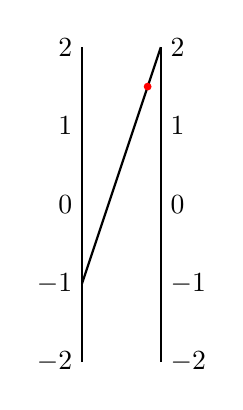
\begin{tikzpicture}
      % Draw the y-axes at x = 0 and x = 1
      \draw[thick] (0, -2) -- (0, 2) node[above] {};
      \draw[thick] (1, -2) -- (1, 2) node[above] {};

      % Add labels for the y-axis ticks
      \foreach \y in {-2, -1, 0, 1, 2} {
          \node[left] at (0, \y) {$\y$};
          \node[right] at (1, \y) {$\y$};
      }

      \draw[thick] (0,-1) -- (1,2) node {};
      \node[circle,fill,color=red,inner sep=1pt] at (0.833, 1.5) {};
    \end{tikzpicture}
    \caption{Check final line for an intersection}
  \end{subfigure}


  \caption{Line representation of the equation \(\delta_\infty((0,0,0) + t(-2,0,3), (-2,-1,1)) = 1.5\)}
  \label{fig:chebyshev_algo}
\end{figure}

\begin{algorithm}[ht]
  \DontPrintSemicolon
  \KwData{vectors \(u, v, w \in \R^d\), \(\varepsilon > 0\)}
  \BlankLine
  \(candidates \gets \set{(2i, u_i - w_i, v_i - u_i), (2i+1, w_i - u_i, u_i - v_i) | i = 0, \dots, d - 1}\) \;
  \(queue \gets PriorityQueue()\) \;
  \(list \gets Array(|candidates|)\) \;
  sort candidates according to second component descendingly,
  in case of ties use the third component as tie breaker descendingly \;
  \(PREV \gets 0, NEXT \gets 1\) \tcp{constants for readability}
  \(curr \gets -1\) \;
  \For{\((i, a, b) \in candidates\)}{
    \If{\(curr = -1\)} {
      \(curr \gets i, a' \gets a, b' \gets b\)\;
      \(list[curr] \gets (-1, -1, a, b)\) \;
      \Continue
    } 

    \If{\( a' + b' \geq a + b\)}{
      \Continue \tcp{new line fully below current line so never maximum}
    } 

    \(list[curr][NEXT] \gets i, list[i] \gets (curr, -1, a, b)\) \;
    \(intersection \gets \frac{a' - a}{b - b'}\) \tcp{always in \([0,1]\)}
    \(queue.insert\_with\_priority((curr, i), intersection)\) \;
    \(curr \gets i, a' \gets a, b' \gets b\) \;
  }

  \caption{chebyshev\_solver\_initialization(\(u, v, w\))}
  \label{algo:solve_chebyshev_init}
\end{algorithm}

\begin{algorithm}[ht]
  \DontPrintSemicolon
  \KwData{vectors \(u, v, w \in \R^d\), \(\varepsilon > 0\)}
  \KwResult{Solution to \cref{eq:solve_chebyshev}}
  \BlankLine
  \(chebyshev\_solver\_initialization(u, v, w)\) \;
  \(last\_intersection \gets 0\) \;
  \While{\(\lnot queue.empty()\)}{
    \((i, j), intersection \gets queue.poll()\) \;
    \If{\(list[i][PREV] = -1 \lor list[j][PREV] = -1\)}{
      \Continue \tcp{One of the lines already removed, no intersection}
    } 
    \If{\(i = HEAD\)}{
      \(HEAD \gets j\) \;
      \(\_, \_, a, b \gets list[i]\) \;
      \If{\(b = 0\)}{
        \If{\(a = \varepsilon\) }{
          Mark \(last\_intersection\) as earliest solution or \(intersection\) as last solution \;
        }
        \(last\_intersection \gets intersection\) \;
        \Continue 
      }
      \(solution \gets \frac{\varepsilon - a}{b}\) \;
      Mark \(solution\) as earliest or last solution if \(solution \in [last\_intersection, intersection]\) \;
      \(last\_intersection \gets intersection\) \;
      \Continue
    }
    \(before_i \gets list[i][PREV]\) \;
    \(list[before_i][NEXT] \gets j, list[j][PREV] \gets before_i\) \;
    \(list[i][PREV] \gets -1\) \tcp{mark as removed}
    \(last\_intersection \gets intersection\) \;
    \If{\(before_i \neq HEAD\)}{
      \(\_, \_, a, b \gets list[j]\) \;
      \(\_, \_, a', b' \gets list[before_i]\) \;
      \(intersection \gets \frac{a' - a}{b - b'}\) \tcp{also in \([0,1]\)}
      \(queue.insert\_with\_priority((before_i, j), intersection)\) \;
    }
  }
  Check for solution in \([last\_intersection, 1]\) \;

  \caption{chebyshev\_solver(\(u, v, w, \varepsilon\))}
  \label{algo:solve_chebyshev}
  
\end{algorithm}

\subsection{\(\O(k^*n^5)\) Algorithm}
\label{subsec:simple_algo}

In this subsection we will sketch \citeauthor{on_optimal_polyline_simplification_using_the_hausdorff_and_frechet_distance}'s algorithm for polyline simplification as well as a simplified version of \citeauthor{computing_the_frechet_distance_between_two_polygonal_curves}'s algorithm to decide if two polylines have Fréchet distance of at most \(\varepsilon\). 

\subsubsection{Fréchet Distance Decision Algorithm}
\label{ssec:alt_godau}
The simplification algorithm we will describe heavily uses a subroutine to solve the following problem: Given \(\varepsilon > 0\), a polyline \(P \) of length \(p\), a polyline segment \(P[j' + t' \dots j+1]\) and a line segment \(\overline{P(i')P(i)}\) for \(i' < i \leq p, j' \leq j < p\in \N\) and \(t \in [0, 1]\). Decide if there is a \(t' \in [0, 1]\) such that \(\delta^F(P[j' + t' \dots j + t], \overline{P(i')P(i)}) \leq \varepsilon\) and if so determine the smallest such \(t\).  

This can be solved by a simplified version of \citeauthor{computing_the_frechet_distance_between_two_polygonal_curves}'s algorithm to decide if the Fréchet distance of two polylines is at most \(\varepsilon\). We present the algorithm in the specific form needed for this problem. 

In both cases we require that \(\delta(P(j' + t'), P(i')) \leq \varepsilon\) as the starting points of both polylines must match by definition. If this is not the case we can return that there is no such \(t\). We set \(t_0 \coloneq \hat t_0'(\overline{P(j)P(j+1)}, P(i))\) and \(t_1 \coloneq \hat t_1'(\overline{P(j)P(j+1)}, P(i))\). As the end points must match, we get that \(t \in [t_0, t_1]\). Thus if there is no such interval we can return that there is no solution.

We distinguish the two cases \(j' = j\) and \(j' < j\). 
\begin{enumerate}
  \item[\(j' = j\): ] In this case both \(t'\) and \(t\) lie on the same line segment \(\overline{P(j)P(j+1)}\) (which is the only line segment of the polyline segment). The only constraints on \(t\) are that \(t \in [t', 1]\) and \(t \in [ t_0, t_1]\) which is possible if and only if \(t' \leq t_1\). If this is the case the solution is \(\max(t', t_0)\).

  \item[\(j' < j\): ] In this case we iterate over all points of the polyline segment \(P(k) = P(j'+1), \dots, P(j)\) and compute the solutions \(\hat t_0'(\overline{P(i')P(i)}, P(k)), \hat t_0'(\overline{P(i')P(i)}, P(k))\). We maintain the first reachable point \(t'\) (initially \(0\)) on the line segment \(\overline{P(i')P(i)}\) for these points and test if \(t' \leq \hat t_0'(\overline{P(i')P(i)}, P(k))\). If that is the case we can update it \(t' \gets \max(t', \hat t_0'(\overline{P(i')P(i)}, P(k)))\). If this is not possible at any step we can return that there is no solution. Otherwise, we have fully traversed the line segment and most of the polyline segment. At this point the solution is merely \(t_0\).
\end{enumerate}

\subsubsection{Polyline Simplification Algorithm}
\label{ssec:simple_algo_main}

Here we outline the global polyline simplification algorithm from \citeauthor{on_optimal_polyline_simplification_using_the_hausdorff_and_frechet_distance} which we have implemented and tested for the Euclidean distance, the Manhattan distance, and the Chebyshev distance. 

Similar to the decision problem we use a dynamic program in which we store the earliest reachable points although in a more complicated manner. We construct a three dimensional table \(DP\) with entries in \([0, 1] \cup \set{\infty}\) for each triple \((k, i, j)\) with \(k, i \in \set{0, \dots, n}\) and \(j \in \set{0, \dots, n - 1}\) where \(n\) is the length of the given polyline \(P\). 

Each entry \(DP[k, i, j]\) stores the smallest \(t \in [0, 1]\) s.t. there is a simplification \(Q\) of \(P[0 \dots i]\) with exactly \(k\) line segments with \(\delta^F(Q, P[0\dots j + t]) \leq \varepsilon\). If no such \(t\) exists we store \(\infty\) in that entry. 
The solution is the smallest \(k^*\) s.t. \(DP[k^*, n, n - 1]\) exists, i.e., there is a simplification \(Q\) of the whole polyline with \(k^*\) many line segments that has \(\delta^F(Q, P[0\dots n - 1 + t]) \leq \varepsilon\) for some \(t \in [0, 1]\) so we can complete the simplification by simply going from \(n-1+t\) to \(n\) on the last line segment of \(P\) while staying on the last point of the simplification. 

For \(k = 0\) it is trivial to compute the entries. If \(i > 0\) we can store \(\infty\) as it is impossible to create a simplification of size \(0\) that goes to any point other than the first point. To find \(DP[0, 0, j]\) we only need to compute the distances from \(P(0)\) to the points \(P(j)\) (see \cref{fig:simpl_init}). Until the first \(j\) with \(\delta(P(0), P(j)) > \varepsilon\) we can store \(0\). From the first such \(j\) we store \(\infty\). This is because the simplification only consists of a single point \(P(0)\) thus the condition \(\delta^F(Q, P[0\dots j + t]) \leq \varepsilon\) simplifies to \(\delta^F(P[0 \dots 0], P[0 \dots j + t])\) and as we cannot move on the single point \(P(0)\) the earliest reachable point on each line segment must be \(t = 0\). 

The correctness of this initialization can be shown rather easily. 
\begin{lemma}
  Let \(P = \angl{P(0)}\) a polyline consisting of a single point and \(Q\) be a polyline of size \(n\). Then \(\delta^F(P, Q) \leq \varepsilon\) if, and only if, \(\delta(P(0), Q(i)) \leq \varepsilon\) for all \(i \in \set{0, \dots, n}\). 
\end{lemma}
\begin{proof}
  For \(\Rightarrow\) we must have some functions \(f,q\) with \(\delta(P(f(t)), Q(g(t))) \leq \varepsilon\) for all \(t\in [0,1]\) where \(f(0) = g(0) = 0\) and \(f(1) = 0\), \(g(1) = n\) and \(f\) and \(g\) are  monotone, meaning that \(\delta(P(0), Q(g(t))) \leq \varepsilon\). As \(g\) is continuous and \(g(0) = 0 \leq g(1) = n\) there must be some \(t \in [0,1]\) with \(g(t) = x\) for any \(x\in \set{0, \dots, n}\).
  
  For \(\Leftarrow\) we show that every point on \(Q\) has distance at most \(\varepsilon\) from \(P(0)\) thus we can choose any suitable function \(g\) (for \(f:[0,0] \to [0,0]\) there is only one possibility). This follows directly from property 3 from \cref{lem:distance_properties} applied to all individual line segment on \(Q\).
\end{proof}

\begin{figure}[b]
    \centering
    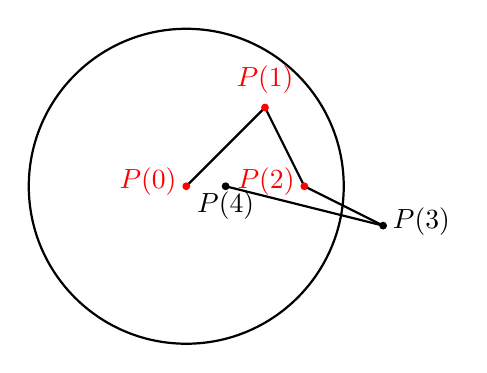
\begin{tikzpicture}[scale=0.5]
        % Define points
        \coordinate (p0) at (0, 0);

        \coordinate (p1) at (2, 2);
        \coordinate (p2) at (3, 0);

        \coordinate (p3) at (5, -1);
        \coordinate (p4) at (1, 0);

        \draw[thick] (p0) -- (p1);
        \draw[thick] (p1) -- (p2);
        \draw[thick] (p2) -- (p3);
        \draw[thick] (p3) -- (p4);

        \draw[thick] (p0) circle (4);

        \node[circle,fill,color=red,inner sep=1pt,label={[text=red, left]:\(P(0)\)}] at (p0) [] {}; 
        \node[circle,fill,color=red,inner sep=1pt,label={[text=red, above]:\(P(1)\)}] at (p1) [] {}; 
        \node[circle,fill,color=red,inner sep=1pt,label={[text=red, left]:\(P(2)\)}] at (p2) [] {}; 
        \node[circle,fill,color=black,inner sep=1pt,label={[text=black, right]:\(P(3)\)}] at (p3) [] {}; 
        \node[circle,fill,color=black,inner sep=1pt,label={[text=black, below]:\(P(4)\)}] at (p4) [] {}; 

    \end{tikzpicture}
  \caption{Initialization of the simplification algorithm for \(k = 0, i = 0\). Only the points in the circle until \(P(2)\) are reachable.}
  \label{fig:simpl_init}
\end{figure}


As for the other entries, the authors show that the entry \(DP[k, i, j]\) can be computed by the minimization over all \(i' < i\) and \(j' \leq j\). We lookup the value \(t \coloneq DP[k-1, i', j']\) and test if there is a \(t' \in [0, 1]\) s.t. \(\delta^F(P[j' + t' \dots j + t], \overline{P(i')P(i)}) \leq \varepsilon\) and return the smallest such \(t\) if possible. This can be done with the algorithm from \citeauthor{computing_the_frechet_distance_between_two_polygonal_curves} with the mentioned modifications. Among all those candidates \(t\) we choose the minimal one. If no such \(t\) exists we can store \(\infty\).

\begin{algorithm}[ht]
  \DontPrintSemicolon
  \KwData{Polyline \(P\) of length \(n\), \(\varepsilon > 0\)}
  \KwResult{Smallest \(\varepsilon\)-simplification of \(P\)}
  \BlankLine
  \(DP \gets Array((n + 1, n + 1, n))\) initialized with \(\infty\) \;
  \For{\(j = 0, \dots, n\)}{
    \If{\(\delta(P(0), P(j)) > \varepsilon\)}{
      \Break
    }
    \(DP[0, 0, j] \gets 0\)
  }
  \For{\(k=1,\dots\) until \(DP[k, n, n-1] \neq \infty\)}{
    \For{\(i=0,\dots, n\)}{
      \For{\(j=0,\dots, n-1\)}{
        \For{\(i' < i\)}{
          \For{\(j' \leq j\)}{
            Let \(t' \gets DP[k-1, i', j']\)\;
            Let \(t \gets AltGodau(P[j' + t' \dots j + 1], \overline{P(i')P(i)}, \varepsilon)\)\;
            \(DP[k, i, j] \gets min(DP[k, i, j], t)\)
          }
        }
      }
    }
  }
  \caption{PolylineSimplification(\(P, \varepsilon\))}
  \label{algo:simplify_simple}
\end{algorithm}

There are \(\O(k^* n^2)\) many iterations to fill in the table and each entry requires \(\O(n^2)\) many computations to find the minimum. Each call to the \(AltGodau\) subroutine requires linear runtime thus in total we have \(\O(k^*n^5)\) run time.

\subsection{Examples}
Before going into possible optimizations, we want to go through an example for the algorithm as well as the \citeauthor{computing_the_frechet_distance_between_two_polygonal_curves} subroutine. This gives us more intuition for the algorithms as well as ideas for further optimizations. Because of cubic amount of entries it is unreasonable to show all computations thus we only show the computations that lead to the simplification and the subroutine for them. 

\begin{figure}
  \centering
  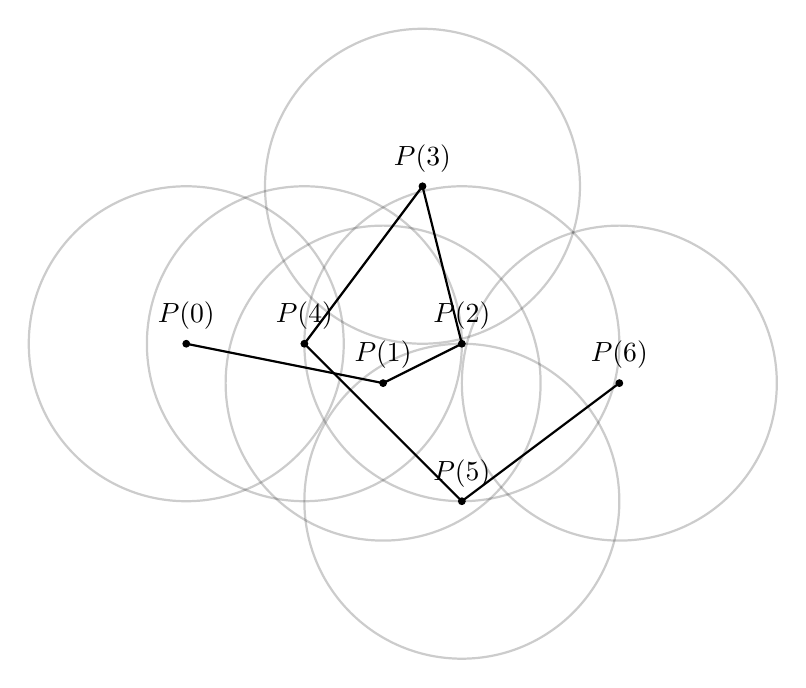
\begin{tikzpicture}[scale=0.5]
    \foreach \i/\x/\y in {0/0/0, 1/5/-1, 2/7/0, 3/6/4, 4/3/0, 5/7/-4, 6/11/-1}{
      \coordinate (p\i) at (\x, \y);
      \node[circle,fill,color=black,inner sep=1pt,label={[text=black, above]:\(P(\i)\)}] at (p\i) [] {}; 
      \draw[thick, opacity=0.2] (p\i) circle (4);
    }
    \foreach \i in {0,...,5}{
      \pgfmathsetmacro{\next}{\i+1}
      \draw[thick] (p\i) -- (p\next);
    }
  \end{tikzpicture}
  \caption{Example polyline with circles with radius \(\varepsilon\) drawn around all points. We note the following relations which may be hard to notice: \(\delta(P(2), P(4)) = \delta(P(2), P(5)) = \varepsilon\), \(\delta(P(2), P(3)) > \varepsilon\), \(\delta(P(2), P(6)) > \varepsilon\).}
  \label{fig:poly-ex-main}
\end{figure}

For the polyline and \(\varepsilon\) in \cref{fig:poly-ex-main} we initialize the table layer for \(k = 0\) by only setting the value \(DP[0,0,0]\) to \(0\) as \(\delta(P(0), P(1)) > \varepsilon\). Even though \(\delta(P(0), P(4)) \leq \varepsilon\) the value \(DP[0,0,4]\) is \(\infty\) as there are points between that already fail.

For the layer \(k = 1\) we can only procede from the entry \(DP[0,0,0] = 0\) as it is the only one we found on the previous layer. All triples \(k, i, j\) for which a valid entry in \([0, 1]\) can be found for the layer \(k = 1\) are listed in \cref{tab:exlayer1}. The respective \(i', j'\) and \(t'\) are not listed as there is only one possible entry.
\begin{table}[ht]
\centering
\begin{tabular}{|ccc|}
\hline
$(1,1,0)$ & $(1,1,1)$ & $(1,1,2)$ \\
$(1,2,0)$ & $(1,2,1)$ & $(1,2,2)$ \\
$(1,2,3)$ & $(1,2,4)$ & $(1,2,5)$ \\
$(1,3,2)$ & $(1,3,3)$ & $(1,4,0)$ \\
$(1,4,1)$ & $(1,4,2)$ & $(1,5,0)$ \\
$(1,5,1)$ & $(1,5,2)$ & \\
\hline
\end{tabular}
\caption{Valid entries for layer \(k = 1\). All procede from \((0,0,0)\).}
\label{tab:exlayer1}
\end{table}

Let us explicitly go through the AltGodau subroutine for the entry \((1, 2, 3)\). i.e., A simplification consisting of one line segment for the polyline \(P[0\dots 2]\) that has distance of at most \(\varepsilon\) to \(P[j' + t'\dots j + t] = P[0 \dots 3 + t]\) where \(t\) is gotten from the subroutine. We consider the line segment \(\overline{P(i')P(i)} = \overline{P(0)P(2)}\) and the polyline segment \(P[j' + t' \dots j + 1] = P[0 \dots 4]\) and perform the algorithm. 

\begin{figure}
  \centering
  \begin{subfigure}[b]{0.4\textwidth}
    \begin{tikzpicture}[scale=0.4]
      \foreach \i/\x/\y in {0/0/0, 1/5/-1, 2/7/0, 3/6/4, 4/3/0, 5/7/-4, 6/11/-1}{
        \coordinate (p\i) at (\x, \y);
        \node[circle,fill,color=black,inner sep=1pt,label={[text=black, above]:\(P(\i)\)}] at (p\i) [] {}; 
      }
      \foreach \i in {0,...,5}{
        \pgfmathsetmacro{\next}{\i+1}
        \draw[thick] (p\i) -- (p\next);
      }

      \path[name path=line] (p0) -- (p2);
      \path[name path=circle] (p1) circle (4);
      \path[name intersections={of=line and circle, by={t0,t1}}];

      \draw[thick, opacity=0.2] (p1) circle (4);
      \draw[color=red, dotted, thick] (p0) -- (p2);
      \draw[color=blue, thick] (p0) -- (p1);
      \draw[color=blue, thick] (p0) -- (t0);
    \end{tikzpicture}
  \end{subfigure}
  \begin{subfigure}[b]{0.4\textwidth}
    \begin{tikzpicture}[scale=0.4]
      \foreach \i/\x/\y in {0/0/0, 1/5/-1, 2/7/0, 3/6/4, 4/3/0, 5/7/-4, 6/11/-1}{
        \coordinate (p\i) at (\x, \y);
        \node[circle,fill,color=black,inner sep=1pt,label={[text=black, above]:\(P(\i)\)}] at (p\i) [] {}; 
      }
      \foreach \i in {0,...,5}{
        \pgfmathsetmacro{\next}{\i+1}
        \draw[thick] (p\i) -- (p\next);
      }

      \path[name path=line] (p0) -- (p2);
      \path[name path=circle1] (p1) circle (4);
      \path[name intersections={of=line and circle1, by={t00,t10}}];
      \path[name path=circle2] (p2) circle (4);
      \path[name intersections={of=line and circle2, by={t01,t11}}];

      \draw[thick, opacity=0.2] (p2) circle (4);
      \draw[color=red, dotted, thick] (p0) -- (p2);
      \draw[color=blue, thick] (p1) -- (p2);
      \draw[color=blue, thick] (t00) -- (t01);
    \end{tikzpicture}
  \end{subfigure}\\
  \begin{subfigure}[b]{0.4\textwidth}
    \begin{tikzpicture}[scale=0.4]
      \foreach \i/\x/\y in {0/0/0, 1/5/-1, 2/7/0, 3/6/4, 4/3/0, 5/7/-4, 6/11/-1}{
        \coordinate (p\i) at (\x, \y);
        \node[circle,fill,color=black,inner sep=1pt,label={[text=black, above]:\(P(\i)\)}] at (p\i) [] {}; 
      }
      \foreach \i in {0,...,5}{
        \pgfmathsetmacro{\next}{\i+1}
        \draw[thick] (p\i) -- (p\next);
      }
      \path[name path=line] (p0) -- (p2);
      \path[name path=circle1] (p2) circle (4);
      \path[name intersections={of=line and circle1, by={t00,t10}}];
      \path[name path=circle2] (p3) circle (4);
      \coordinate (t01) at (6,0);

      \draw[thick, opacity=0.2] (p3) circle (4);
      \draw[color=red, dotted, thick] (p0) -- (p2);
      \draw[color=blue, thick] (p2) -- (p3);
      \draw[color=blue, thick] (t00) -- (t01);
    \end{tikzpicture}
  \end{subfigure}
  \begin{subfigure}[b]{0.4\textwidth}
    \begin{tikzpicture}[scale=0.4]
      \foreach \i/\x/\y in {0/0/0, 1/5/-1, 2/7/0, 3/6/4, 4/3/0, 5/7/-4, 6/11/-1}{
        \coordinate (p\i) at (\x, \y);
        \node[circle,fill,color=black,inner sep=1pt,label={[text=black, above]:\(P(\i)\)}] at (p\i) [] {}; 
      }
      \foreach \i in {0,...,5}{
        \pgfmathsetmacro{\next}{\i+1}
        \draw[thick] (p\i) -- (p\next);
      }
      % same point
      \coordinate (t00) at (6,0);
      \path[name path=line] (p3) -- (p4);
      \path[name path=circle] (p2) circle (4);
      \path[name intersections={of=line and circle, by={t0,t1}}];

      \draw[thick, opacity=0.2] (p2) circle (4);
      \draw[color=red, dotted, thick] (p0) -- (p2);
      \draw[color=red, thick] (p3) -- (t0);
      \draw[color=blue, thick] (t00) -- (p2);
    \end{tikzpicture}
  \end{subfigure}
  \caption{Finding the first reachable point on \(\overline{P(3)P(4)}\). Resulting in \(t = 0.04\) marginally below point \(P(3)\). Note again that \(\delta(P(2), P(3)) > \varepsilon\). The point \(P(4)\) is not part of the simplification, it only lies on the line segment \(\overline{P(0)P(2)}\) by chance.}
  \label{fig:poly-ex-123-ag}
\end{figure}

From \(DP[1,2,3] = 0.04\) we can procede to the end of the polyline to get a simplification of size \(2\) as seen in \cref{fig:poly-ex-265-ag}. A simplification of size \(1\) is not possible as that would be the line segment \(\overline{P(0)P(6)}\) but there is no point on that line segment that has distance \(\leq \varepsilon\) from \(P(3)\). 

\begin{figure}
  \centering
  \begin{subfigure}[b]{0.4\textwidth}
    \begin{tikzpicture}[scale=0.4]
      \foreach \i/\x/\y in {0/0/0, 1/5/-1, 2/7/0, 3/6/4, 4/3/0, 5/7/-4, 6/11/-1}{
        \coordinate (p\i) at (\x, \y);
        \node[circle,fill,color=black,inner sep=1pt,label={[text=black, above]:\(P(\i)\)}] at (p\i) [] {}; 
      }
      \foreach \i in {0,...,5}{
        \pgfmathsetmacro{\next}{\i+1}
        \draw[thick] (p\i) -- (p\next);
      }

      \path[name path=line] (p3) -- (p4);
      \path[name path=circle] (p2) circle (4);
      \path[name intersections={of=line and circle, by={t0,t1}}];

      \draw[thick, opacity=0.2] (p4) circle (4);
      \draw[color=red, dotted, thick] (p2) -- (p6);
      \node[circle,fill,color=blue,inner sep=1pt] at (p2) [] {}; 
      \draw[color=blue, thick] (t0) -- (p4);
    \end{tikzpicture}
  \end{subfigure}
  \begin{subfigure}[b]{0.4\textwidth}
    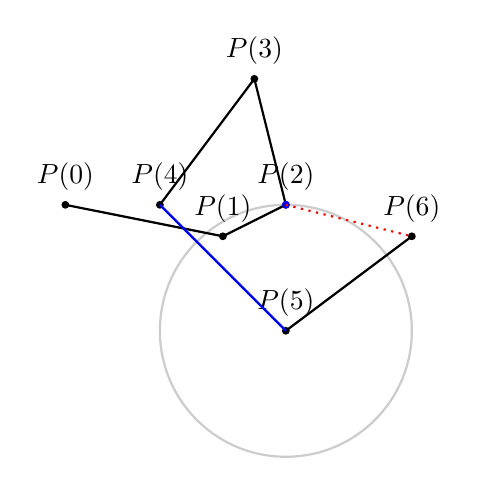
\begin{tikzpicture}[scale=0.4]
      \foreach \i/\x/\y in {0/0/0, 1/5/-1, 2/7/0, 3/6/4, 4/3/0, 5/7/-4, 6/11/-1}{
        \coordinate (p\i) at (\x, \y);
        \node[circle,fill,color=black,inner sep=1pt,label={[text=black, above]:\(P(\i)\)}] at (p\i) [] {}; 
      }
      \foreach \i in {0,...,5}{
        \pgfmathsetmacro{\next}{\i+1}
        \draw[thick] (p\i) -- (p\next);
      }

      \node[circle,fill,color=blue,inner sep=1pt] at (p2) [] {}; 
      \draw[thick, opacity=0.2] (p5) circle (4);
      \draw[color=red, dotted, thick] (p2) -- (p6);
      \draw[color=blue, thick] (p4) -- (p5);
    \end{tikzpicture}
  \end{subfigure}\\
  \begin{subfigure}[b]{0.4\textwidth}
    \begin{tikzpicture}[scale=0.4]
      \foreach \i/\x/\y in {0/0/0, 1/5/-1, 2/7/0, 3/6/4, 4/3/0, 5/7/-4, 6/11/-1}{
        \coordinate (p\i) at (\x, \y);
        \node[circle,fill,color=black,inner sep=1pt,label={[text=black, above]:\(P(\i)\)}] at (p\i) [] {}; 
      }
      \foreach \i in {0,...,5}{
        \pgfmathsetmacro{\next}{\i+1}
        \draw[thick] (p\i) -- (p\next);
      }
      \path[name path=line] (p5) -- (p6);
      \path[name path=circle] (p6) circle (4);
      \path[name intersections={of=line and circle, by={t0,t1}}];

      \draw[thick, opacity=0.2] (p6) circle (4);
      \draw[color=blue, thick] (p2) -- (p6);
      \draw[color=blue, thick] (p5) -- (t0);
    \end{tikzpicture}
  \end{subfigure}
  \caption{Finding the first reachable point on \(\overline{P(5)P(6)}\). With that we have found a simplification for the whole polyline.}
  \label{fig:poly-ex-265-ag}
\end{figure}

We can also convince ourselves that the solution must be correct as the application of the algorithm from \citeauthor{computing_the_frechet_distance_between_two_polygonal_curves} guarantees that the Fréchet distance is at most \(\varepsilon\) by construction and even yields the points that can be used to construct suitable functions that show this. Further, the simplification must be optimal as it has size two so the only possible smaller one would have size one. This is not possible as the only such simplification would be the line segment \(\overline{P(0)P(6)}\) but no point on that line segment is reachable from \(P(3)\) with a distance of at most \(\varepsilon\) thus it cannot be a valid simplification.

For completeness sake the entries on the layer \(k = 2\) are listed in \cref{tab:exlayer2}. The entry \((k - 1, i', j')\) they reference from the previous layer is added after the tuple. This predecessor tuple is not necessarily unique, in fact, every single one of these has at least two different possibilities for \(i', j'\).
\begin{table}[ht]
\centering
\begin{tabular}{|ccc|}
\hline
$(2,4,3):(2, 1)$ & $(2,4,4):(2, 1)$ & $(2,5,4):(2,4)$ \\
$(2,5,5):(2,4)$ & $(2,6,5):(2,4)$ & \\
\hline
\end{tabular}
\caption{Valid entries for layer \(k = 1\). All procede from \((0,0,0)\).}
\label{tab:exlayer2}
\end{table}

\subsection{Optimizations}
\label{ssec:optimizations}
Based on the just described algorithm we outline optimizations that greatly reduce the \(\O(k^*n^5)\) runtime in practice or improve upon the algorithm in terms of space and numerical stability. The most effective optimizations circumvent the theoretical runtime by skipping iterations. 

We first note that for the entry \((k, i, j)\) in the dynamic program we do not always need to iterate over all possible \(i' < i\) and \(j' \leq j\). As we are interested in the minimal value \(t\) on the line segment \(\overline{v_{j}v_{j+1}}\) that can be reached, we can stop further search if we have reached a lower bound for that value. Such a lower bound is \(\hat t_0'(\overline{v_{j}v_{j+1}}, i)\), i.e. the modified solution to the \cref{eq:eq_solve_main}, which is tight as for a sufficiently large \(k\) this value must be reached eventually. This allows an early break out of the search through the \(i' < i, j'\leq j\) and a speed up of upto quadratic runtime. 

Another optimization based on a similar insight is the following: If the entry at \((k-1, i, j) = \hat t_0'(\overline{v_{j}v_{j+1}}, i)\), i.e., we have found a simplification for the same \(i\) and \(j\) that has already reached the optimal value, we know this cannot be improved in the current layer \(k\) or any further one. This means, the entry at \((k, i, j)\) can never be used by some entry \((k + 1, i'', j'')\) because of minimality as any such entry that uses \((k, i, j)\) could have already used \((k-1, i, j)\) for \((k, i'', j'')\). This allows us to completely ignore the computation of the value. This allows a continuous speed up of the algorithm while it runs as once this happens for an entry, it will happen for all further ones with a higher value of \(k\) so with each layer more entry computations can be skipped. 

Another way to skip computations is to ignore all \(i\) with \(i < k\) as well as all \(i'\) with \(i' < k - 1\) in the computations as there can never be a simplification of \(P[0\dots i]\) that uses more than \(i\) line segments thus it must always hold that \(i \geq k\). 

A last simple optimization of a similar type which is particularly useful for well-behaved polylines is to not even start the iterations over the \(i', j'\) if there is no solution \(\hat t_0'(\overline{v_{j}v_{j+1}}, i)\). This happens often if there are not too many line segments close to each other.











%\subsection{Cubic Runtime Algorithm}
%\label{subsec:refined_algo}

\subsection{Implementation}
\label{subsec:implementation}
% details 
% only use min(p, q) space instead of p * q space for decision variant (especially for our case constant extra space)
%


